\section{手先加速度をあげるために再設計したロボットの解析}\label{ux624bux5148ux52a0ux901fux5ea6ux3092ux3042ux3052ux308bux305fux3081ux306bux518dux8a2dux8a08ux3057ux305fux30edux30dcux30c3ux30c8ux306eux89e3ux6790}

ここでは,手先加速度をあげるために軽量化を行うべく再設計したロボットアームの解析を行う.

解析の手順は,基準となるロボットの解析をした時と同じである.

\subsection{手先加速度をあげるために再設計したロボットの構造解析}\label{ux624bux5148ux52a0ux901fux5ea6ux3092ux3042ux3052ux308bux305fux3081ux306bux518dux8a2dux8a08ux3057ux305fux30edux30dcux30c3ux30c8ux306eux69cbux9020ux89e3ux6790}

ここでは,手先加速度を上げるために再設計したロボットの構造解析を行う.

\subsubsection{慣性モーメントの解析}\label{ux6163ux6027ux30e2ux30fcux30e1ux30f3ux30c8ux306eux89e3ux6790}

SolidEdgeを使って求めたリンクアームの体積,質量,慣性モーメントに加え,材質と密度をまとめて記載したものが表\ref{light-robot-data}である.有効数字は4桁とした.

\begin{table}[htb]
\caption[]{リンクアームの各値}
  \begin{center}
    \begin{tabular}{|c|c|} \hline
      材質 & アルミニウム1060 \\ \hline
      密度 [$\rm kg/m^3$]& 2712 \\ \hline
      体積[$\rm m^3$] & 0.1195 \\ \hline
      質量[kg] & 324.1 \\ \hline
      慣性モーメント & 576.4 [$\rm kg m^2$] \\ \hline
    \end{tabular}
    \label{light-robot-data}
  \end{center}
\end{table}

まず,慣性モーメントについて考える.

基準となるロボットとは異なり,形状が複雑となり,慣性モーメントを求めるのが複雑であるので,慣性モーメントの理論値とシミュレーションによって求めた慣性モーメントの値の大小関係が一致しているかという点でシミュレーション結果の妥当性を考える.

今回の手先加速度をあげるために再設計したロボットのアームについて,重心軸周りの慣性モーメント\(I_G\)は\(175.9[\rm kgm^2]\)となった.

ゆえに,軸間距離\(d=1.105[\rm m]\),重心周りの慣性モーメント\(I_G=176.0[\rm kgm^2]\)及び質量\(M=324.1[\rm kg]\)を使い,平行軸の定理より慣性モーメントを求めると式\ref{solveLightKansei}となる.

\begin{eqnarray}
  I &=& I_G+d^2M \nonumber \\
    &=& 176.0 + 1.105^{2} \cdot 324.1 \nonumber \\
    &=& 571.7
  \label{solveLightKansei}
\end{eqnarray}

となり,平行軸の定理を使って求めた慣性モーメントの値\(I=571.7[\rm kgm^2]\)はSolidEdgeの解析機能を使って求めた慣性モーメントの値\(I=576.4[\rm kgm^2]\)ものとほぼ一致する.

また,手先加速度をあげるために再設計したロボットは,基準ロボットから直方体を切り抜いたものであるので,慣性モーメント及び質量は小さくなっていることが予想される.

基準ロボットと今回手先加速度を上げるために再設計したロボットの各値を比較したのが表\ref{compare-basic-light-mass}である.

\begin{table}[htb]
\caption[]{リンクアームの各値}
  \begin{center}
    \begin{tabular}{|c|c|c|} \hline
      項目 & 基準アーム & 手先加速度を上げるために再設計したアーム \\ \hline \hline
      体積[$\rm m^3$] & 0.1792 & 0.1195 \\ \hline
      質量[kg] & 485.8 & 324.1 \\ \hline
      慣性モーメント[$\rm kg m^2$] & 751.9 & 576.4 \\ \hline
    \end{tabular}
    \label{compare-basic-light-mass}
  \end{center}
\end{table}

表\ref{compare-basic-light-mass}を見て分かるように,再設計後は体積,質量,慣性モーメントの全てが小さくなっているため,SolidEdgeの解析結果は正しいことが分かる.

\subsubsection{応力の解析}\label{ux5fdcux529bux306eux89e3ux6790}

次に,応力の解析及びその解析結果の検証を行っていく.
手先加速度をあげるために再設計したロボットのアームの応力図を図\ref{light-ouryoku}に示す.

\begin{figure}[htbp]
  \begin{center}
    \begin{tabular}{c}
      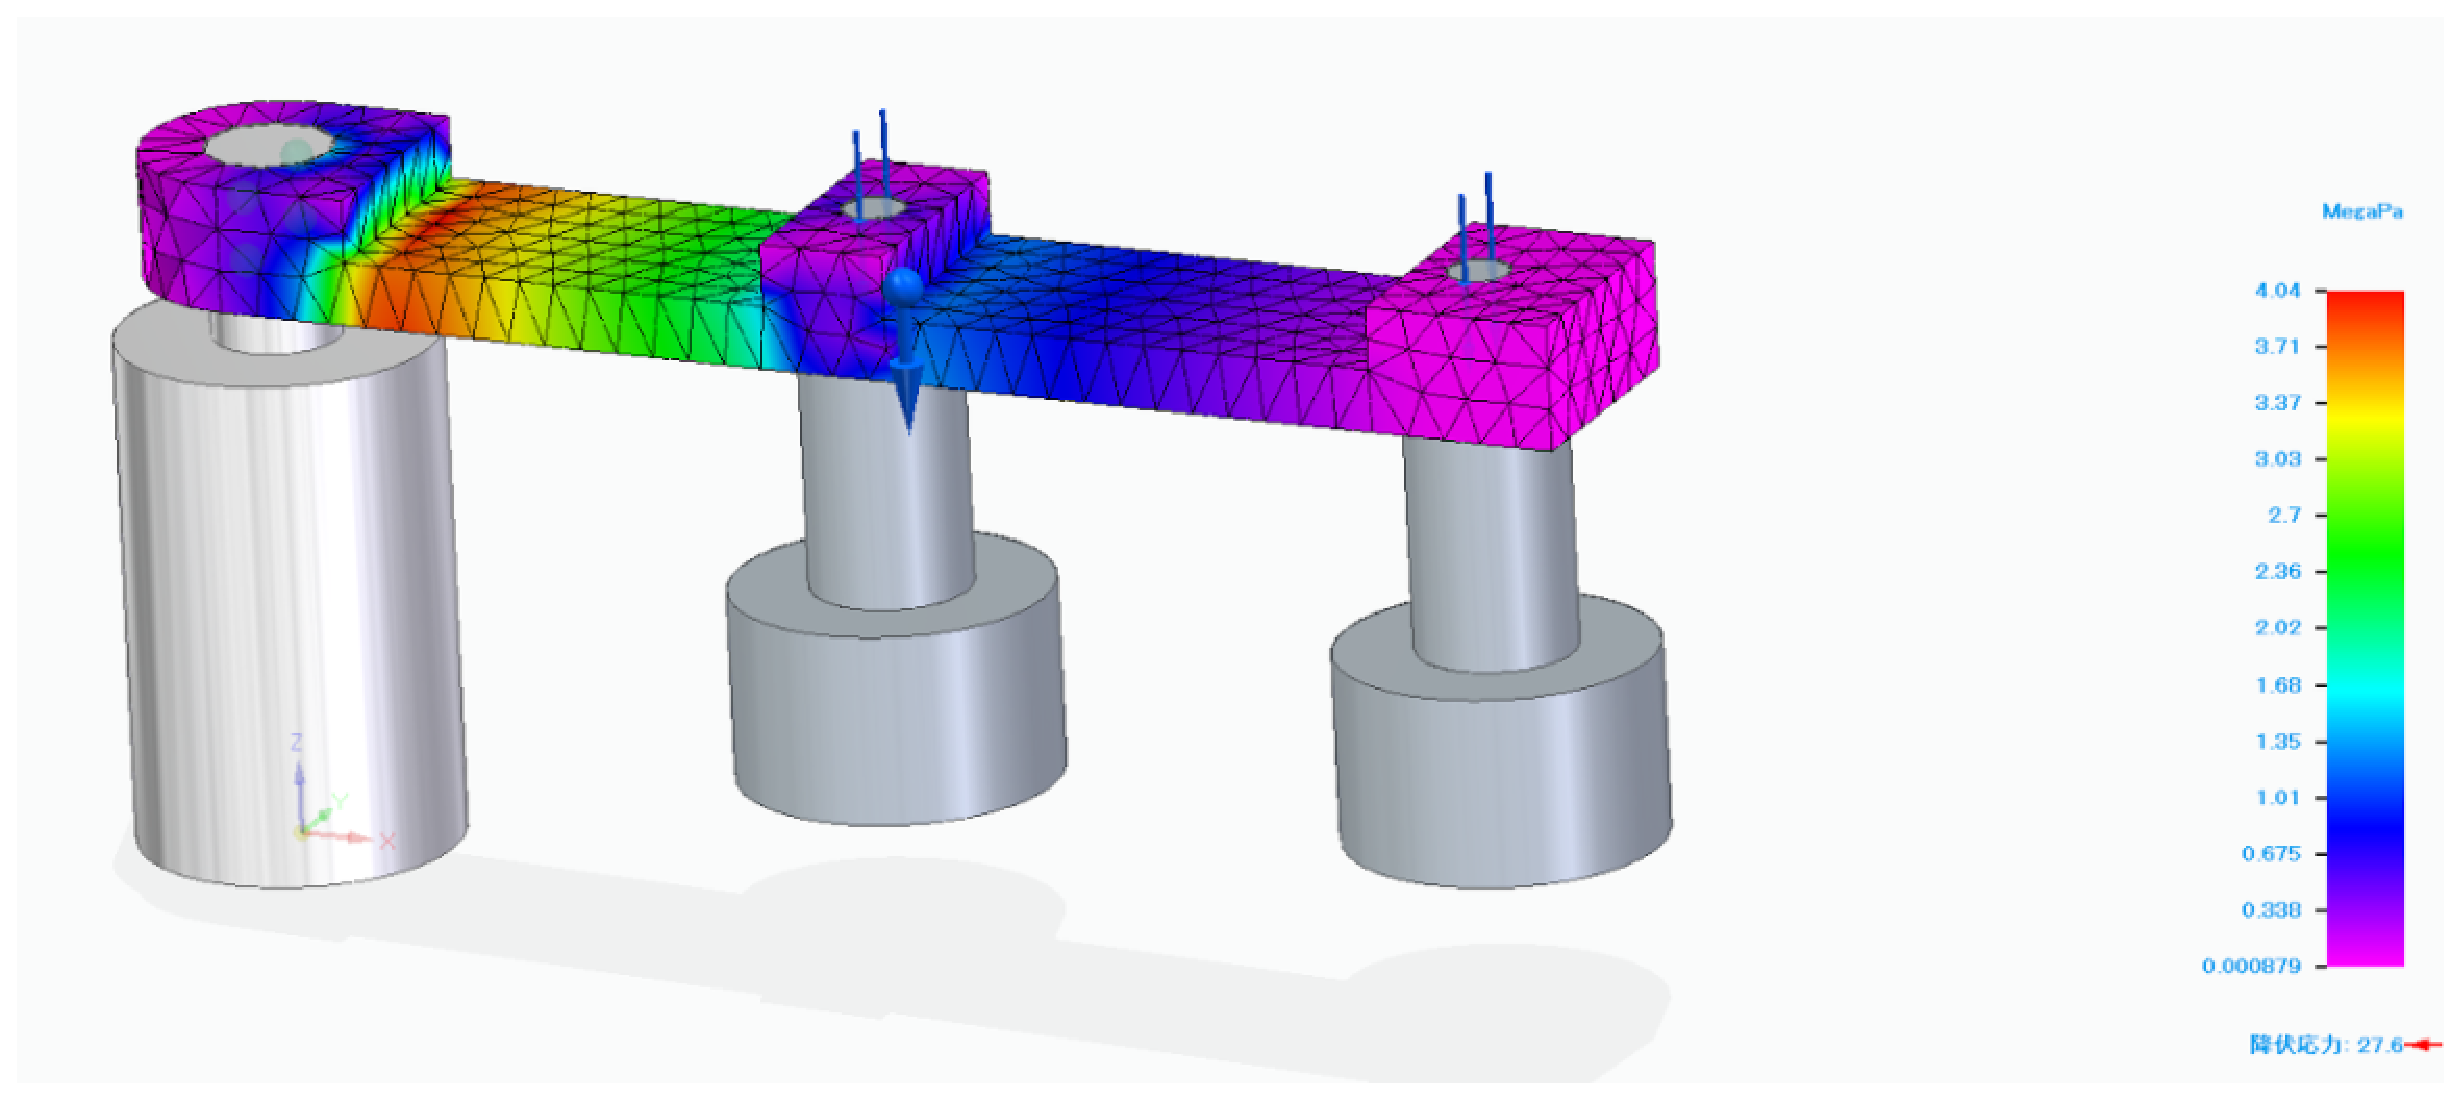
\includegraphics[height=5.0cm]{img/eps/light-ouryoku.eps}
    \end{tabular}
    \caption{手先加速度を重視したロボットの構造解析の応力図}
    \label{light-ouryoku}
  \end{center}
\end{figure}

この時,図\ref{light-ouryoku-result}に示す結果がSolid
Edgeより出力された.

\begin{figure}[htbp]
  \begin{center}
    \begin{tabular}{c}
      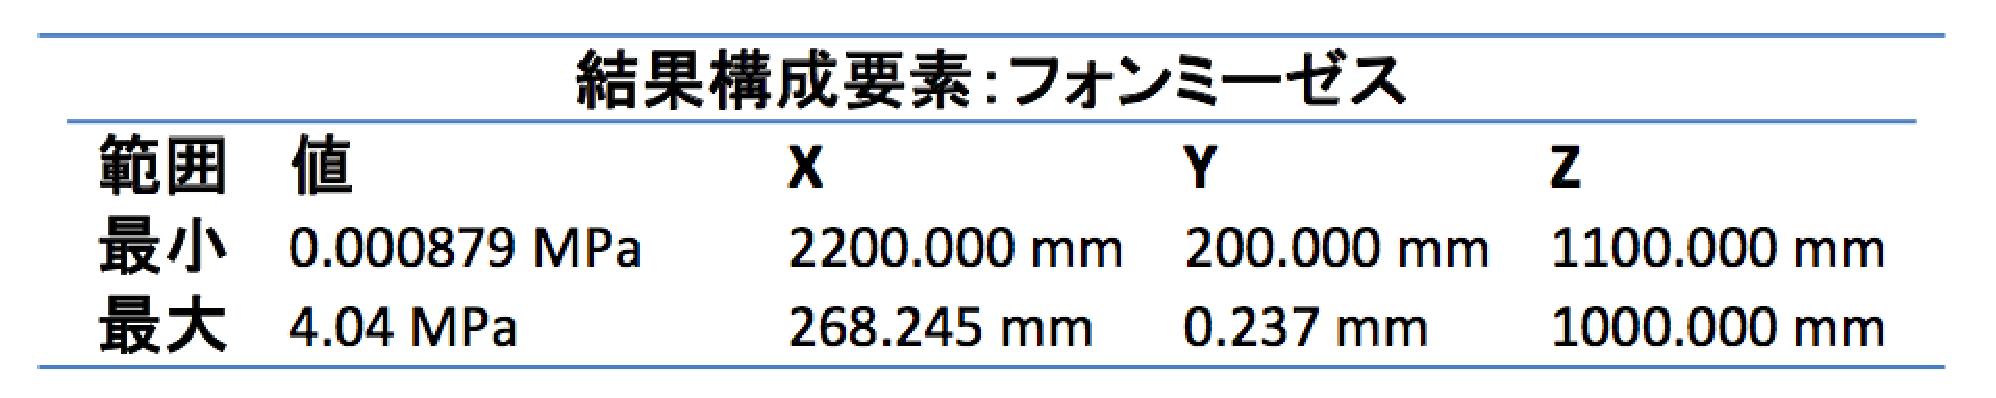
\includegraphics[height=2.2cm]{img/eps/light-ouryoku-result.eps}
    \end{tabular}
    \caption{手先加速度を上げるために再設計したロボットの応力解析結果}
    \label{light-ouryoku-result}
  \end{center}
\end{figure}

Solid Edgeによって得た応力の結果と,解析的に計算した応力の値を比較する.

アームの自重を\(M_{arm}\),回転軸とアームの重心点の距離を\(R_a\),アーム中心部に設置されたブレードの荷重による力を\(F_1\),回転軸とアームの中心部の距離を\(R_{b1}\),アーム先端に設置されたブレードの荷重による力を\(F_2\),回転軸とアーム先端部の距離を\(R_{b2}\)とすると,アームの部分にかかる曲げモーメント\(M\)は式\ref{light-magemoment}で表される.
ただし,重力加速度は\(g\)と置いた.

\begin{eqnarray}
  M &=& M_{arm}g R_a + F_1 R_{b1} + F_2 R_{b2} 
  \label{light-magemoment}
\end{eqnarray}

今回,アームの重さが324.1{[}kg{]}であるので,\(M_{arm}=324.1\),\(g=9.81\),\(R_a=1.03\),\(F_1=F_2=117.7\),\(R_{b1}=1\),\(R_{b2}=2\)を代入すると,式\ref{light-magemoment-calc}となる.このとき,\(R_a\)は先ほど求めた回転軸と重心の軸間距離を使用した.

\begin{eqnarray}
  M &=& M_{arm}g R_a + F_1 R_{b1} + F_2 R_{b2}  \nonumber \\
    &=& 324.1*9.8*1.03 + 1*117.7+2*117.7 \nonumber \\
    &=& 3624
  \label{light-magemoment-calc}
\end{eqnarray}

よって,曲げモーメントMは3624{[}\(\rm kg m^2\){]}となる.

また,今回の断面係数Zは,直方体のY方向長さ\(b=0.4[\rm m]\)と,直方体のZ方向長さ\(h=0.1[\rm m]\)を使って,式\ref{light-danmen-calc}と書ける.

\begin{eqnarray}
  Z &=& \frac{bh^2}{6} \nonumber \\
    &=& \frac{0.4*0.1^2}{6} \nonumber \\
    &=& 0.000667 [\rm m^3]
  \label{light-danmen-calc}
\end{eqnarray}

ここで,応力\(\sigma\)は,断面係数\(Z\)を用いて,式\ref{light-ouryoku}と書ける.

\begin{eqnarray}
  \sigma &=& \frac{M}{Z} \nonumber \\
         &=& 5433883 [\rm Pa]\nonumber \\
         &=& 5.4 [MPa]
  \label{light-ouryoku}
\end{eqnarray}

SolidEdgeを用いて計算した結果は4.04{[}MPa{]}で,理論解は5.4{[}MPa{]}となった.

基準となるロボットアームに比べて今回のロボットは形状が複雑であるので,誤差が大きくなってしまった.

基準となるロボットアームと,今回のロボットの同部位に働いている応力の大小関係を比較することで,今回の応力解析の結果の妥当性を検証する.

図\ref{ouryoku-compare-basic-light}に,基準ロボット及び今回再設計したロボットの応力図の比較を示す.

\begin{figure}[htbp]
  \begin{center}
    \begin{tabular}{c}
      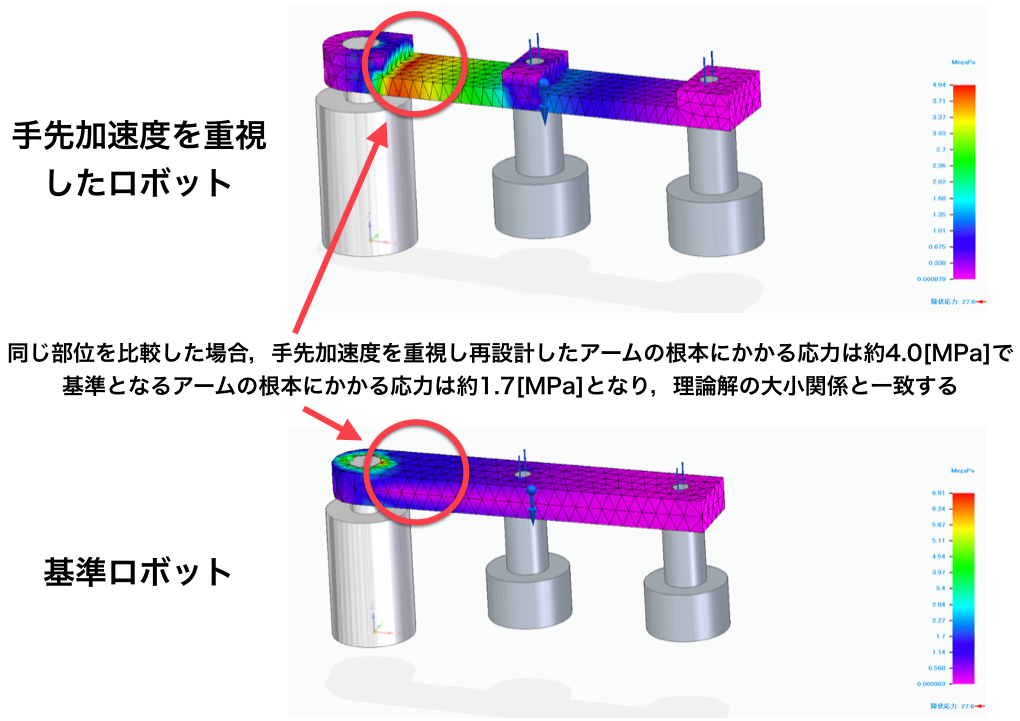
\includegraphics[height=8.5cm]{img/eps/ouryoku-compare-basic-light.eps}
    \end{tabular}
    \caption{同部位にかかる応力の大きさの比較}
    \label{ouryoku-compare-basic-light}
  \end{center}
\end{figure}

今回のロボットは軽量化のためにアームの一部分が細くなっているため,同部位を比べた場合,今回のロボットにかかる応力のほうが大きくなっているはずである.

図\ref{ouryoku-compare-basic-light}で述べた大小関係が理論解と一致している.形状が複雑なので,誤差はあるが大小関係が理論解と一致しているため,今回の解析結果は正しいと判断できる.

基準ロボットの安全率に関して考えたときと同じく,安全率は3を満たすためには,式\ref{basic-anzen}より,許容応力が9.2{[}Mpa{]}であることが分かる.

今回,最大応力は4.04{[}MPa{]}であり,許容応力以下であるため安全率3の基準を満たしているといえる.

\subsubsection{変位の解析}\label{ux5909ux4f4dux306eux89e3ux6790}

次に,重力及び荷重によってかかる変位について解析する.

Solid
Edgeのシミュレーション機能を用いて変位を解析した所,変位分布は図\ref{light-heni}となった.

\begin{figure}[htbp]
  \begin{center}
    \begin{tabular}{c}
      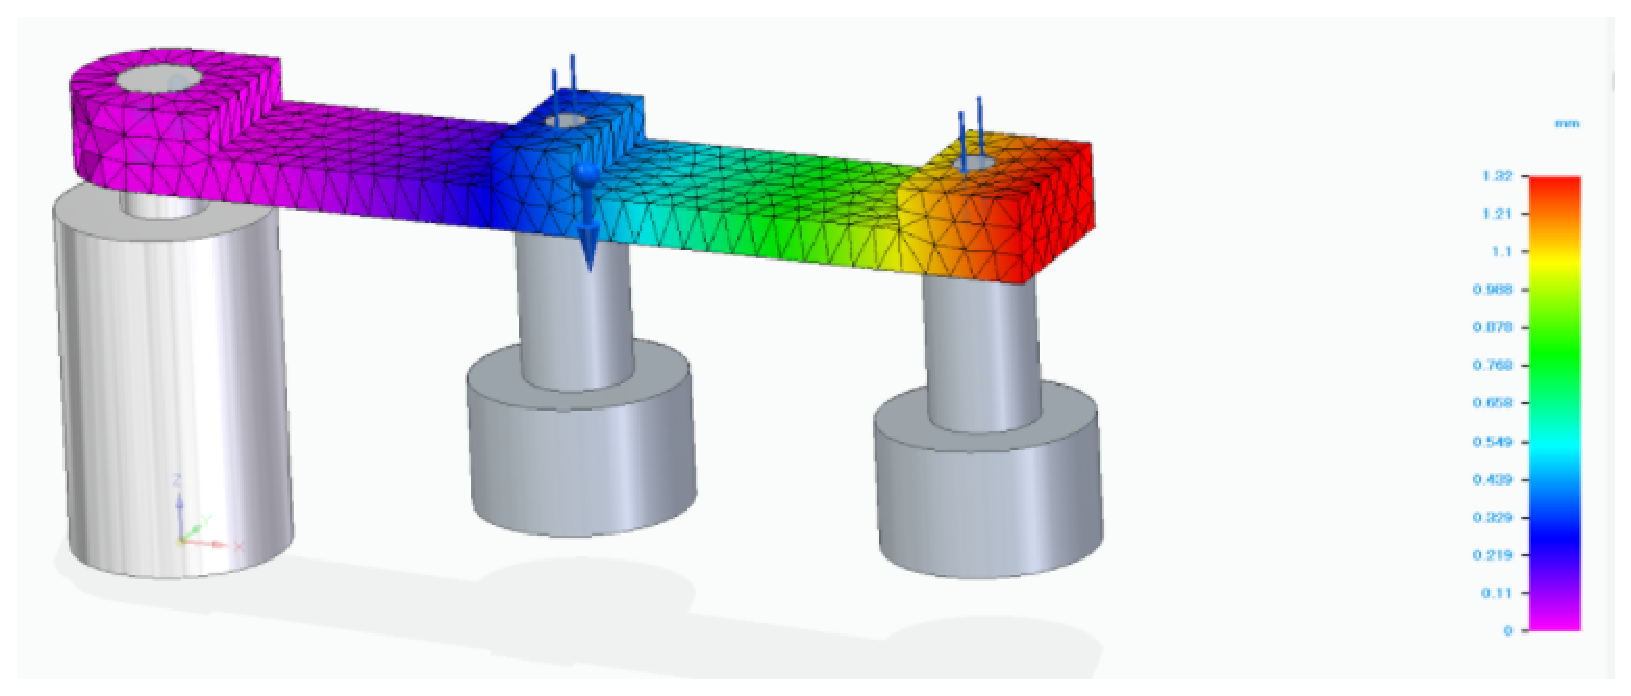
\includegraphics[height=5.5cm]{img/eps/light-heni.eps}
    \end{tabular}
    \caption{手先加速度を上げるために再設計したロボットの変位分布}
    \label{light-heni}
  \end{center}
\end{figure}

この時,図\ref{light-heni-result}に示す変位結果がSolid
dgeより出力された.

\begin{figure}[htbp]
  \begin{center}
    \begin{tabular}{c}
      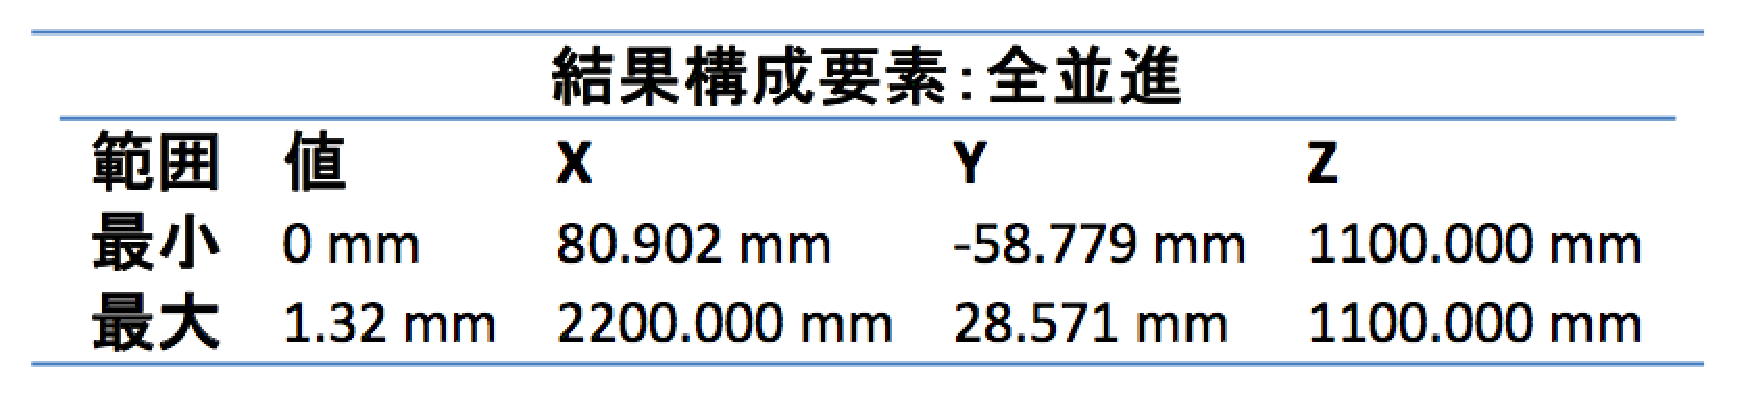
\includegraphics[height=2.5cm]{img/eps/light-heni-result.eps}
    \end{tabular}
    \caption{手先加速度を上げるために再設計したロボットの変位解析結果}
    \label{light-heni-result}
  \end{center}
\end{figure}

基準となるロボットのアームに比べて,手先加速度を上げるために再設計したロボットのアームは細いため,変位が増えていると考えられる.

シミュレーションの結果によると,基準となるロボットアームのZ方向最大たわみは0.541{[}mm{]}であり,手先加速度を上げるために再設計したロボットアームのZ方向最大たわみは1.32{[}mm{]}であるので,たわみの理論解と大小関係が一致する.

よって,変位のシミュレーション結果は正しいと考えられる.

\subsection{手先加速度をあげるために再設計したロボットの機構解析}\label{ux624bux5148ux52a0ux901fux5ea6ux3092ux3042ux3052ux308bux305fux3081ux306bux518dux8a2dux8a08ux3057ux305fux30edux30dcux30c3ux30c8ux306eux6a5fux69cbux89e3ux6790}

ここでは,手先加速度をあげるために再設計したロボットアームの機構解析を行う.

ロボットアームに対して,基準座標系\(\Sigma_0\),リンク座標系\(\Sigma_1\),及び手先座標系\(\Sigma_E\)を記述したのが図\ref{light-tesaki}である.

\begin{figure}[htbp]
  \begin{center}
    \begin{tabular}{c}
      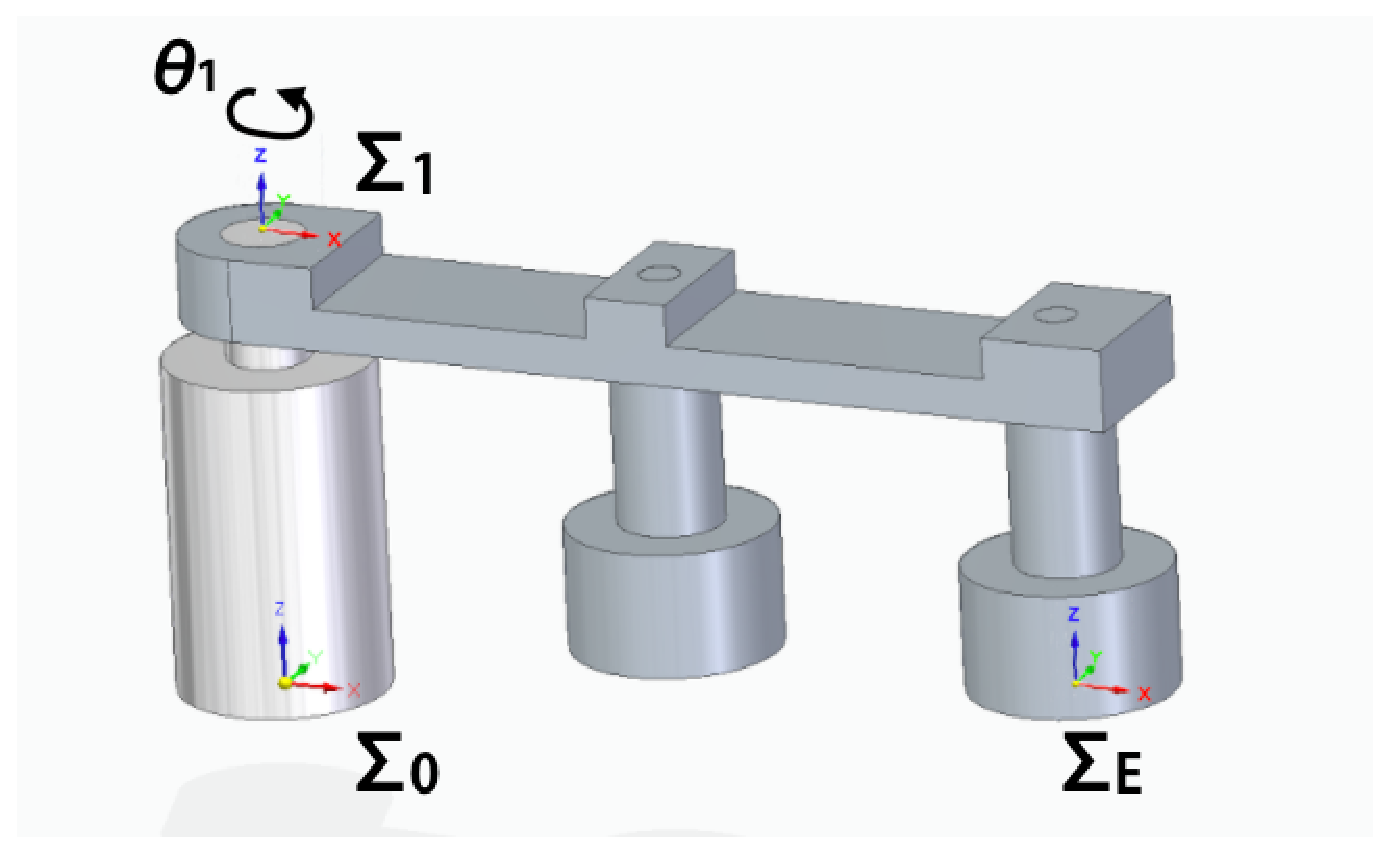
\includegraphics[height=5.5cm]{img/eps/light-dh.eps}
    \end{tabular}
    \caption{手先加速度を重視し再設計したロボットの各種座標系}
    \label{light-tesaki}
  \end{center}
\end{figure}

このロボットアームのリンクパラメータをDH記法を用いて書くと表\ref{light-dh-link}となる.
今回,手先としてアーム先端のブレード部分を選んだ.

\begin{table}[htb]
\caption[]{リンクパラメータ}
  \begin{center}
    \begin{tabular}{|c|c|c|c|c|} \hline
      $i$ & $a_{i-1}$ & $\alpha_{i-1}$ & $d_i$ & $\theta_i$\\ \hline \hline
      1 & 0 & 0 & 1100[mm] & ($\theta_1$) \\ \hline
      2 & 2000[mm] & 0 & -900[mm] & 0 \\ \hline
    \end{tabular}
    \label{light-dh-link}
  \end{center}
\end{table}

次に,関節角度の理論解及びシミュレーション結果を比較する.

SimXpertを使用して,今回作成したアームロボットの関節回転角度を求めた結果を図\ref{strong-kaiten}に示す.

\begin{figure}[htbp]
  \begin{center}
    \begin{tabular}{c}
      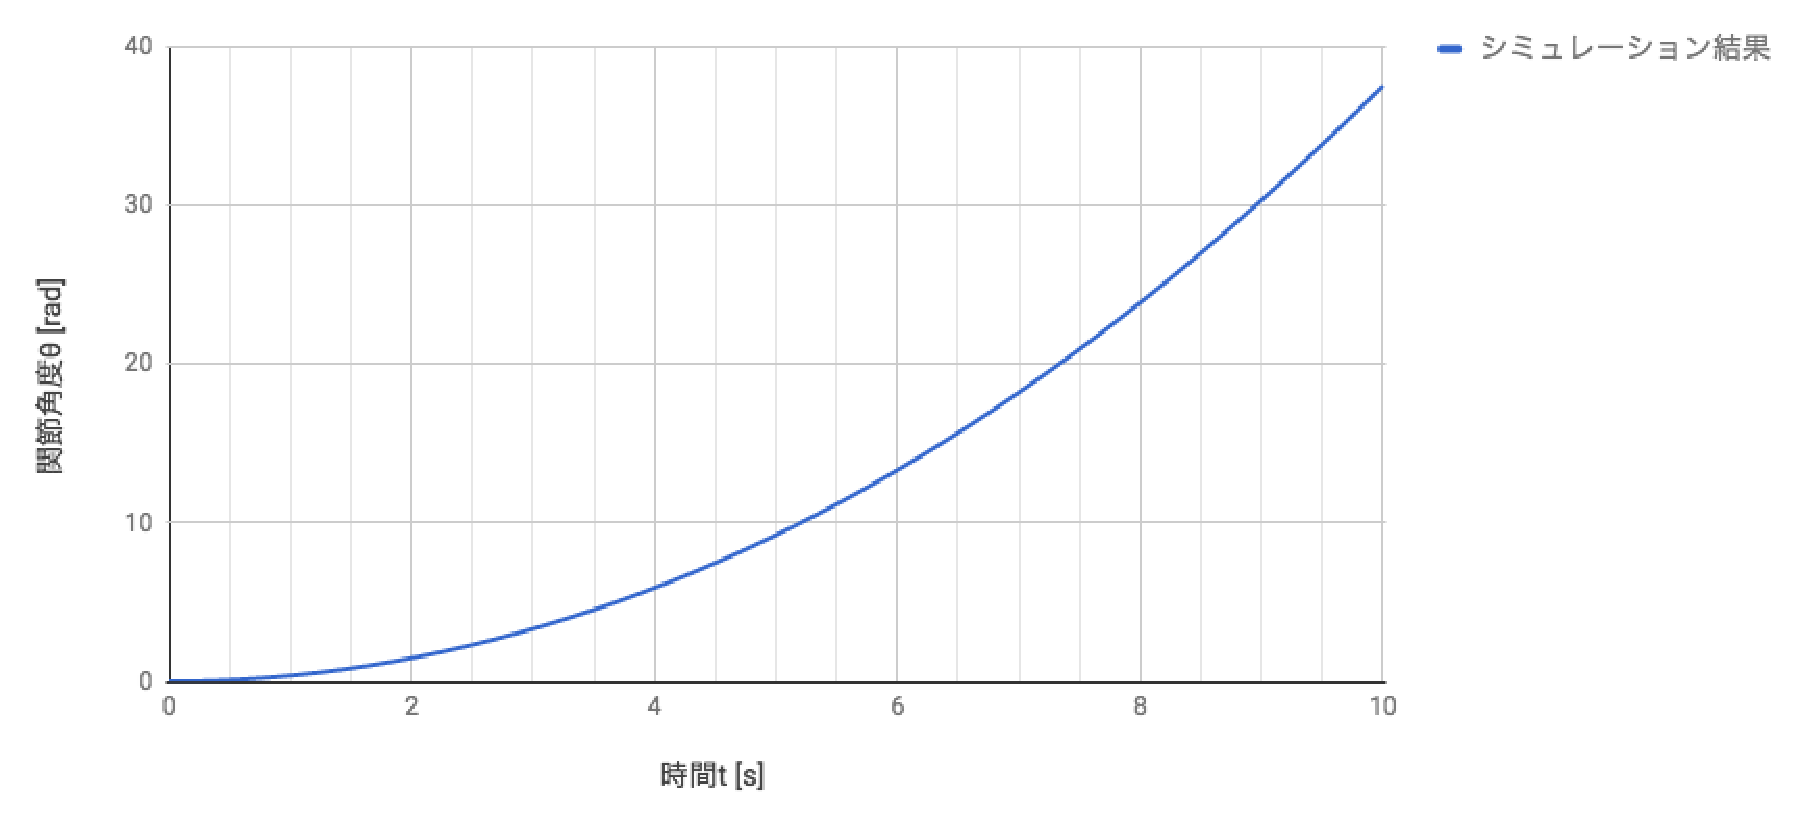
\includegraphics[height=5.5cm]{img/eps/light-kaiten2.eps}
    \end{tabular}
    \caption{手先加速度を上げるために再設計したロボットのアームの関節回転角}
    \label{strong-kaiten}
  \end{center}
\end{figure}

式\ref{kaiten-houteisiki}で示した回転の運動方程式に,関節駆動トルク\(\tau=393\),そして慣性モーメント\(I=576.445\)を代入すると,式\ref{light-kaiten-houteisiki-calc}となる.

\begin{eqnarray}
  393 &=& 576.445 \frac{d^2 \theta}{d t^2}
  \label{light-kaiten-houteisiki-calc}
\end{eqnarray}

式\ref{light-kaiten-houteisiki-calc}は,時間に関する2階微分であるので,角速度及び角度の初期値を0として両辺2度積分することで微分方程式を解くと,式\ref{light-deg}の角度の関数を得る.

\begin{eqnarray}
  \theta = 0.34088t^2
  \label{light-deg}
\end{eqnarray}

式\ref{light-deg}で求めた\(\theta\)に関する式と,SimXpertによって得られたシミュレーション結果を比較したのが図\ref{compare-light}である.

\begin{figure}[htbp]
  \begin{center}
    \begin{tabular}{c}
      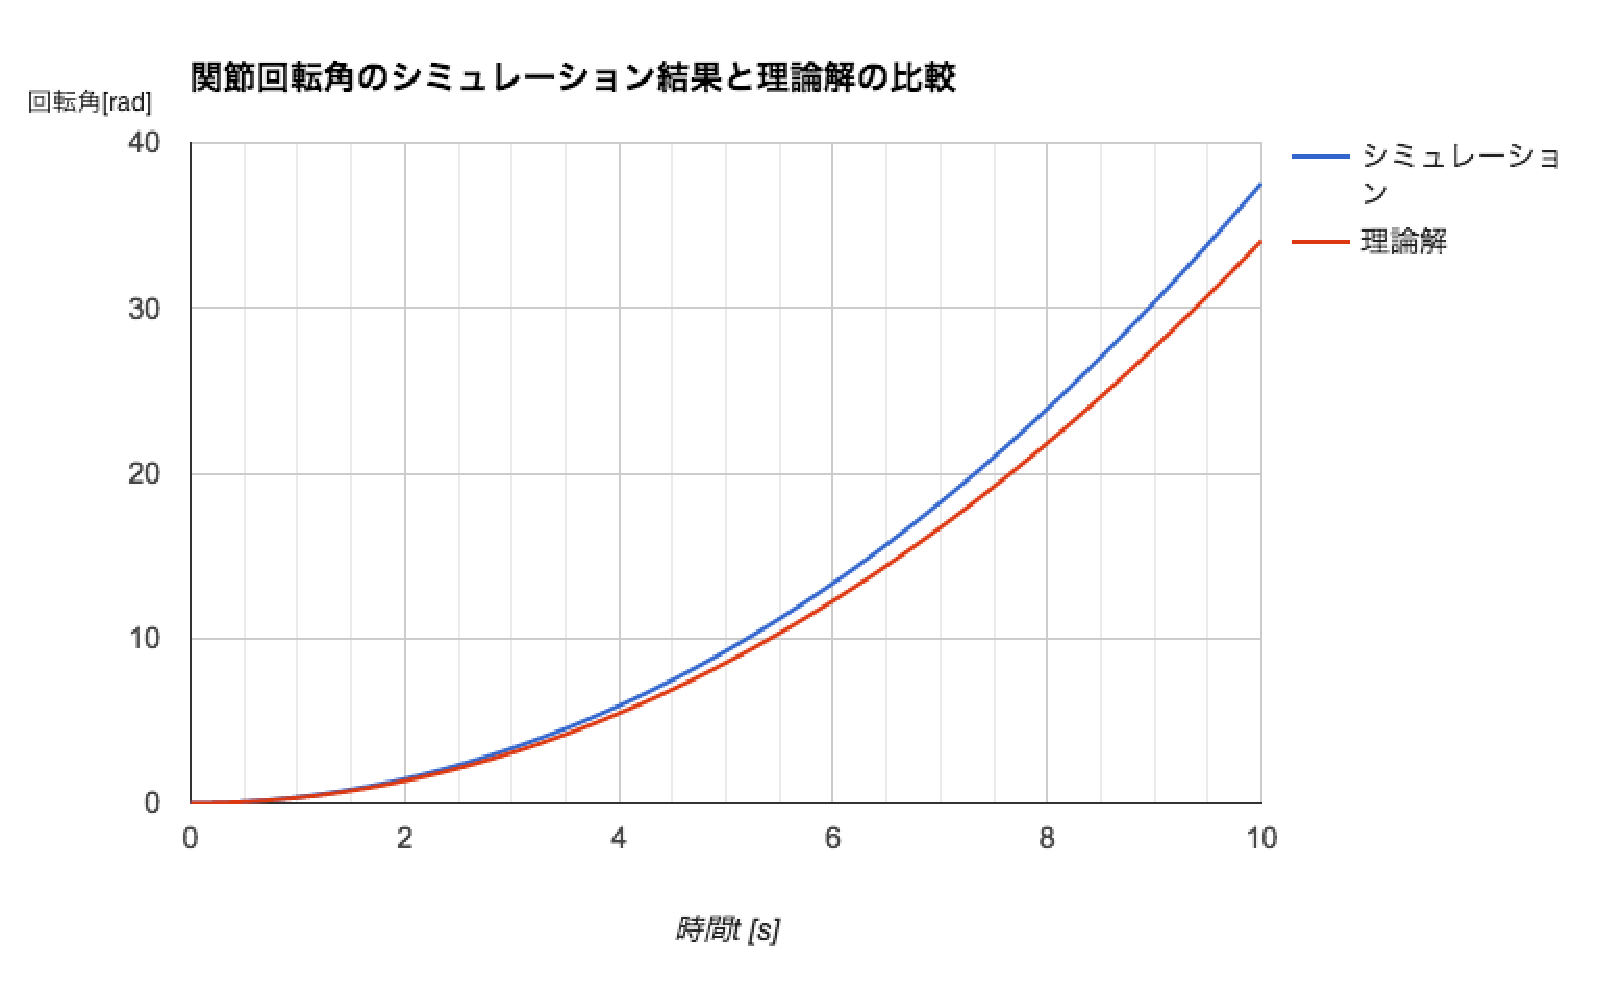
\includegraphics[height=6.5cm]{img/eps/compare-light.eps}
    \end{tabular}
    \caption{シミュレーション結果と理論解の回転角度の比較}
    \label{compare-light}
  \end{center}
\end{figure}

多少の誤差はあるが,図\ref{compare-light}より,シミュレーション結果は正しいことが分かる.

この関節角度のシミュレーション結果を最小二乗法を用いて2次の多項式近似を行うと,式\ref{light-niji-kinji}を得ることが出来る.

\begin{eqnarray}
  \frac{d\theta}{dt} &=& 0.382t^2-0.077t+0.078\nonumber \\
  &\approx& 0.382t^2
  \label{light-niji-kinji}
\end{eqnarray}

式\ref{light-niji-kinji}で得た関節加速度を使用し,手先加速度及び手先速度の理論値を計算し,シミュレーション結果と比較する.

手先加速度に関しては,基準ロボットの手先加速度について考えたときと同様に,手先速度のシミュレーション結果元にして手先加速度を割り出すという方法を取ることにする.

SimXpertより出力された手先速度を図\ref{light-tesaki-sokudo}に示す.この時,青の破線が手先加速度のX方向成分,赤の破線が手先加速度のY方向成分,そして赤の実線が手先加速度のノルムを表している

\begin{figure}[htbp]
  \begin{center}
    \begin{tabular}{c}
      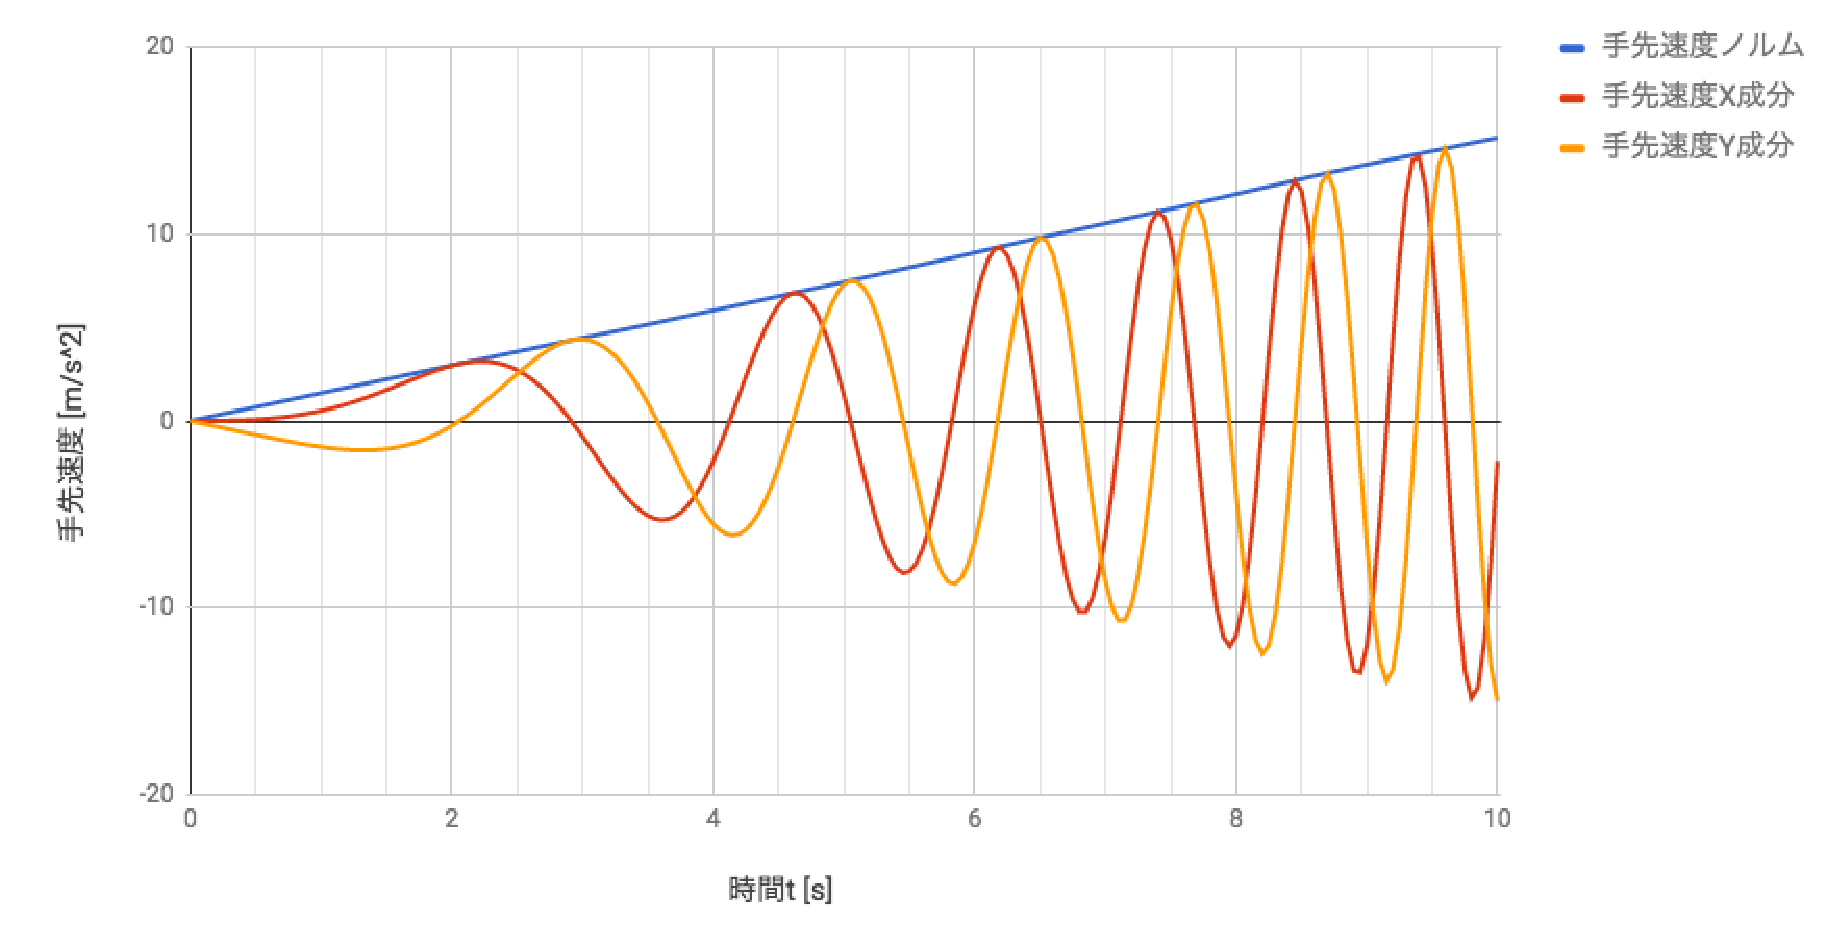
\includegraphics[height=5.5cm]{img/eps/light-tesaki-sokudo2.eps}
    \end{tabular}
    \caption{手先速度のシミュレーション結果}
    \label{light-tesaki-sokudo}
  \end{center}
\end{figure}

次に,この手先速度のシミュレーション結果の妥当性を理論解と比較することで検証する.

先ほど,式\ref{light-deg}で,\(\theta = 0.382t^2\)を得た.

角速度\(\frac{d\theta}{dt}\)は式\ref{light-deg}を両辺\(t\)で時間微分することで得られるため,式\ref{light-ddeg}となる.

\begin{eqnarray}
  \frac{d\theta}{dt} = 0.764t
  \label{light-ddeg}
\end{eqnarray}

ここで,角速度\(\frac{d\theta}{dt}\)と手先速度の大きさ\(v\)の間には,式\ref{hand-vel}の関係がある.ただし,回転中心と手先間の距離を\(r\)と置いた.

\begin{eqnarray}
  v &=& r\frac{d\theta}{dt}
  \label{light-hand-vel}
\end{eqnarray}

式\ref{light-ddeg},及び式\ref{light-hand-vel}より,手先速度の大きさの理論解は式\ref{light-hand-velocity}となる.

\begin{eqnarray}
  v &=& r(0.764t) \nonumber \\
    &=& 2(0.764t) \nonumber \\
    &=& 1.528t
  \label{light-hand-velocity}
\end{eqnarray}

ゆえに,手先速度の理論解は\(v=1.528t\)と求まった.

図\ref{strong-tesaki-sokudo}に示した,SimXpertによる手先速度のシミュレーション結果と,手先速度の理論解を比較したのが図\ref{light-compare-vel}である.

\begin{figure}[htbp]
  \begin{center}
    \begin{tabular}{c}
      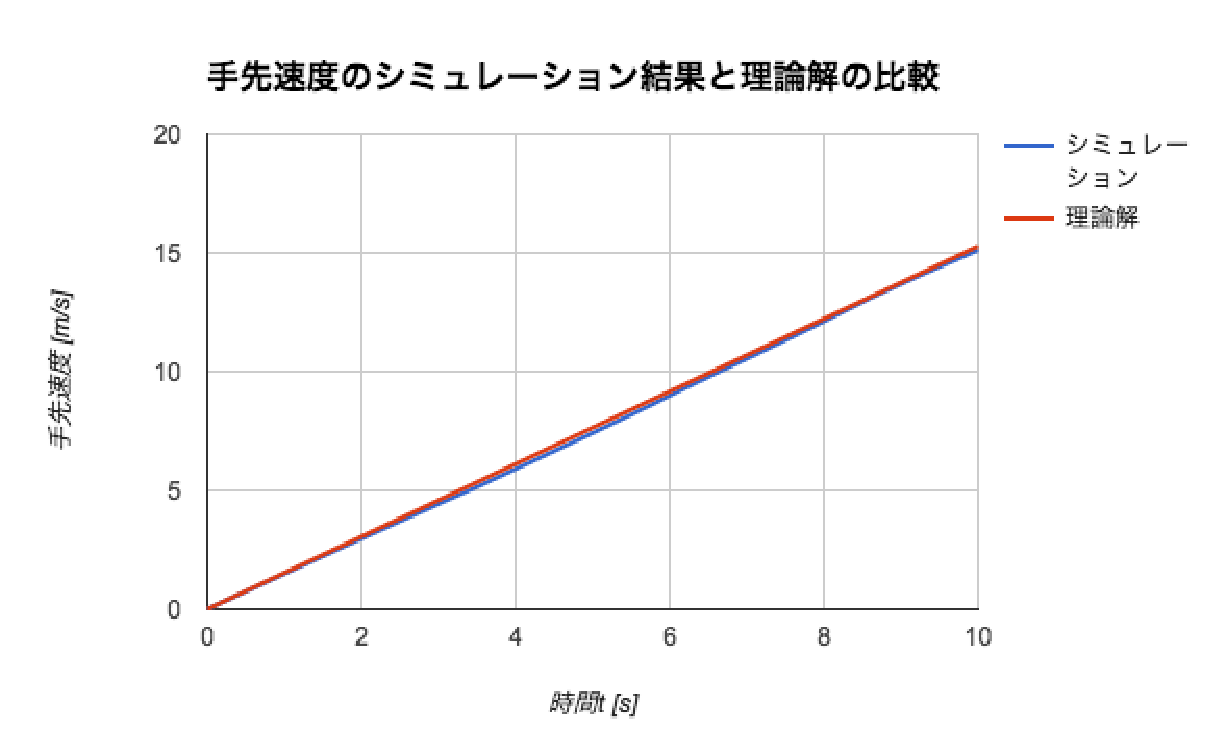
\includegraphics[height=8.5cm]{img/eps/light-compare-vel.eps}
    \end{tabular}
    \caption{手先速度のシミュレーション結果と理論解の比較}
    \label{light-compare-vel}
  \end{center}
\end{figure}

SimXpertによって得られた手先速度のシミュレーション結果を最小二乗法によって1次関数近似を行うと,式\ref{light-teaki-kinji}を得る.

\begin{eqnarray}
 v &=& 1.523t - 0.102 \nonumber \\
 &\approx& 1.523
  \label{light-teaki-kinji}
\end{eqnarray}

手先速度のシミュレーション結果によって得られた式\ref{light-teaki-kinji}と式\ref{light-hand-velocity}の理論解は一致しており,シミュレーション結果が正しいと考えられる.

ここで,この手先速度を時間微分したものが手先加速度であるため,手先加速度として\(1.528[\rm m/s^2]\)を得る.
手先加速度の理論解および数値解のグラフを図\ref{light-acc}に示す.

\begin{figure}[htbp]
  \begin{center}
    \begin{tabular}{c}
      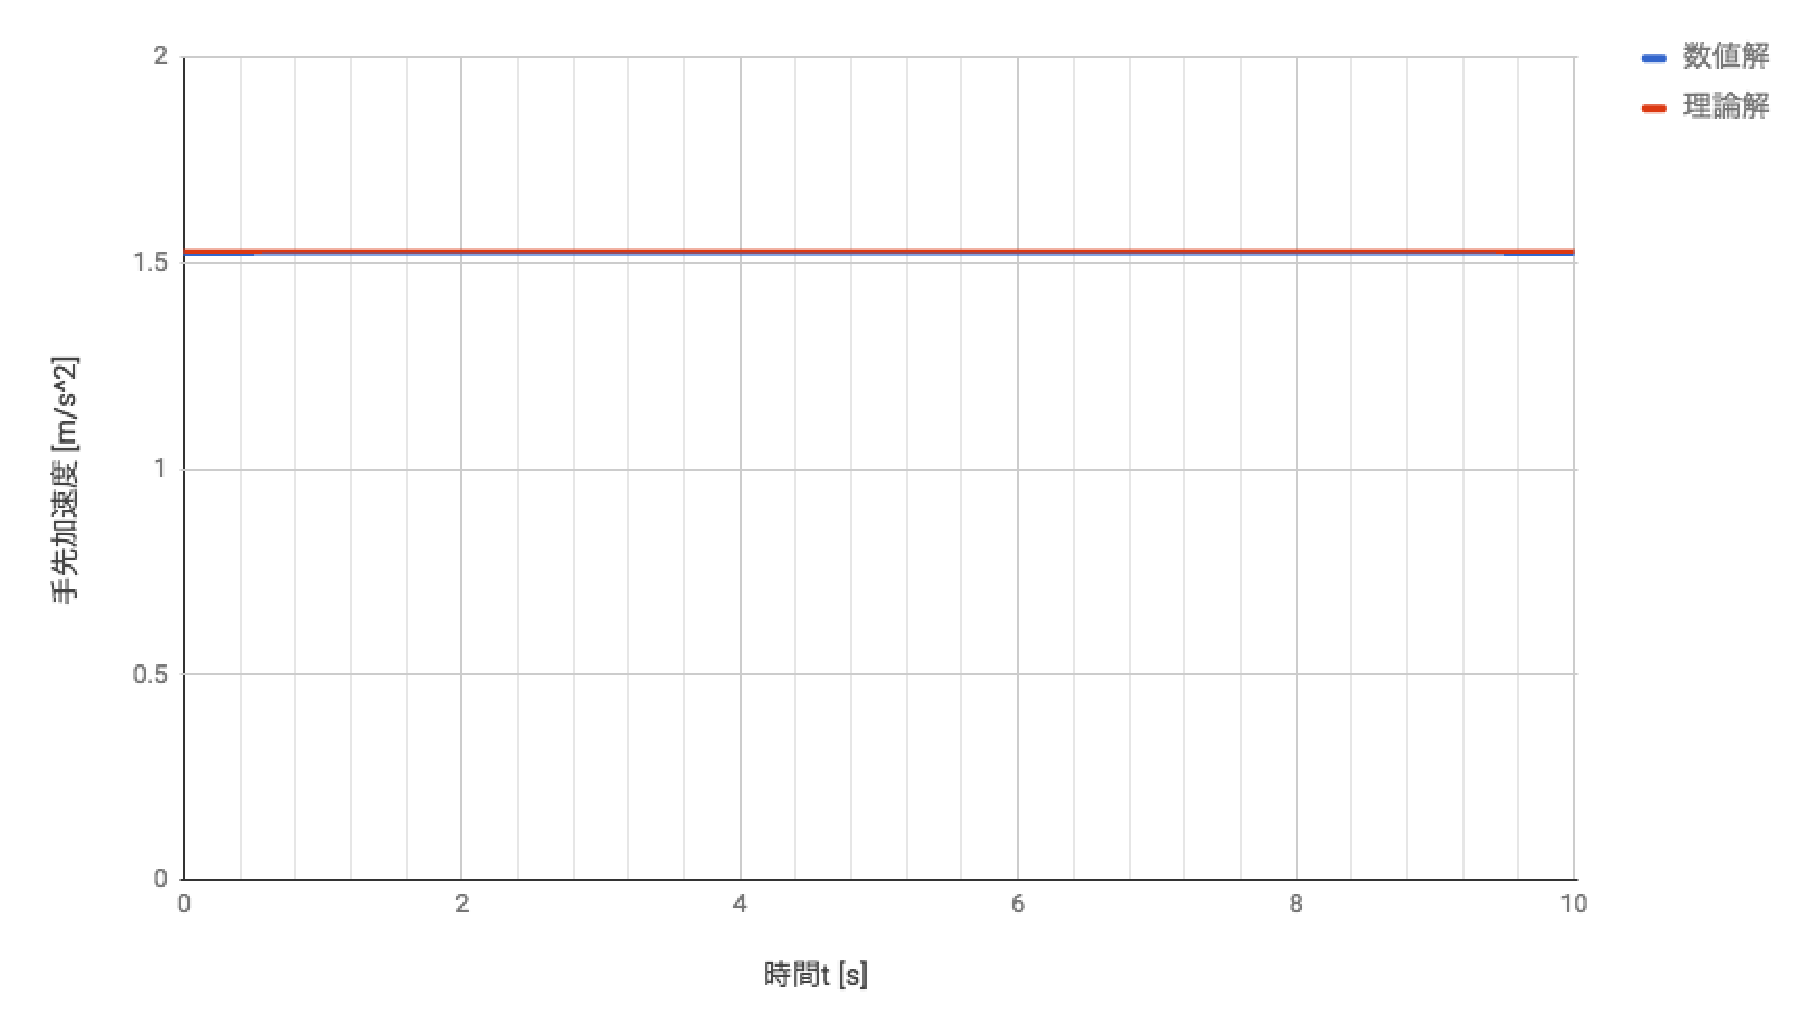
\includegraphics[height=5.5cm]{img/eps/light-acc.eps}
    \end{tabular}
    \caption{手先加速度の理論解と数値解の比較}
    \label{light-acc}
  \end{center}
\end{figure}
